\chapter{Estado del arte}\label{cap:estado_del_arte}

% [En el estado del arte se necesita hacer un estudio tanto sobre la tecnología que soporta el proyecto como sobre el problema que se aborda en él. Se puede estructurar por secciones y se aconseja utilizar referencias a los documentos e información que se describe aquí.]

% [Como norma general y más en proyectos con carácter investigador, se recomienda añadir un párrafo por cada documento/referencia que estudie del estado del arte, finalizando esta sección con un párrafo explicativo de la novedad/característica que propone, modifica o añade el proyecto sobre dicho estado del arte.]

\section{Computación de alto rendimiento (\acs{HPC})}\label{sec:computacion_alto_rendimiento}

La computación de alto rendimiento (\acs{HPC}, por sus siglas en inglés) se refiere a la práctica de agregar poder de cómputo para lograr un rendimiento mucho mayor que el que se podría obtener con una computadora convencional, con el objetivo de resolver problemas complejos en ciencias, ingeniería o negocios \cite{sravanthi2014hpc}.

\subsubsection{Objetivos principales de HPC}

El propósito fundamental de HPC es acelerar la resolución de problemas complejos, alcanzando resultados en tiempos factibles que de otra manera requerirían semanas o meses. Para ello, HPC se apoya en dos conceptos centrales: paralelización y escalabilidad.

\paragraph{Paralelización}
La paralelización consiste en descomponer un problema en múltiples tareas que puedan ejecutarse simultáneamente en distintos núcleos de procesamiento, ya sean CPUs o GPUs. Este enfoque permite aprovechar todos los recursos del sistema para reducir significativamente el tiempo de ejecución de las aplicaciones. Existen distintos niveles de paralelización:

\begin{itemize}
    \item \textbf{Paralelización a nivel de instrucción}: el procesador ejecuta varias instrucciones de manera simultánea mediante pipelines y unidades vectoriales.
    \item \textbf{Paralelización a nivel de hilo o thread}: diferentes hilos de ejecución procesan tareas concurrentes dentro de un mismo núcleo o CPU.
    \item \textbf{Paralelización a nivel de proceso o nodo}: tareas completas se distribuyen entre múltiples nodos de un clúster, cada uno con su propio conjunto de recursos.
\end{itemize}
\paragraph{Escalabilidad}
La escalabilidad se refiere a la capacidad de un sistema para mejorar su rendimiento al añadir más recursos de cómputo. Se distingue entre:

\begin{itemize}
    \item \textbf{Escalabilidad fuerte}: mejora del tiempo de ejecución de un problema de tamaño fijo al incrementar el número de recursos.
    \item \textbf{Escalabilidad débil}: capacidad de mantener constante el tiempo de ejecución al aumentar simultáneamente el tamaño del problema y los recursos de manera proporcional.
\end{itemize}

Lograr buena escalabilidad es crítico, especialmente en entornos multinodo, donde la comunicación entre nodos y la sincronización de tareas pueden generar cuellos de botella.

\subsubsection{Arquitecturas comunes en HPC}

Los sistemas HPC modernos pueden clasificarse en función de su arquitectura:

\begin{itemize}
    \item \textbf{Sistemas homogéneos}: utilizan múltiples CPUs idénticas interconectadas. Esto simplifica la planificación de tareas y el balance de carga, aunque no aprovecha posibles ventajas de eficiencia energética de núcleos especializados.
    \item \textbf{Sistemas heterogéneos}: combinan distintos tipos de núcleos de procesamiento o aceleradores especializados, como GPUs, FPGAs o núcleos de eficiencia energética tipo \textit{big.LITTLE}. Estas arquitecturas permiten un mayor rendimiento por watt y mejor aprovechamiento de recursos, pero requieren técnicas avanzadas de programación y planificación.
    \item \textbf{Clústeres y supercomputadores}: integran múltiples nodos interconectados mediante redes de alta velocidad (Infiniband, Omni-Path). Soportan aplicaciones distribuidas que requieren comunicación intensiva entre nodos, siendo los supercomputadores clústeres de alto rendimiento con características avanzadas de interconexión, memoria y almacenamiento.
\end{itemize}

\subsection{Virtualización vs contenerización}\label{subsec:virtualizacion_contenedores}

La virtualización y la contenerización representan dos enfoques distintos para la abstracción y gestión de recursos computacionales, cuyo propósito es ejecutar aplicaciones de manera aislada del sistema operativo anfitrión. Ambas tecnologías han sido ampliamente utilizadas en entornos de servidores y, más recientemente, en la computación de alto rendimiento (\acs{HPC}), aunque presentan diferencias fundamentales que influyen en el rendimiento, la eficiencia y la portabilidad.

\subsubsection{Máquinas virtuales (VMs)}

Las máquinas virtuales permiten la ejecución de sistemas operativos completos sobre un hipervisor, el cual actúa como intermediario entre el hardware físico y el sistema operativo invitado. Cada VM incorpora su propio kernel, librerías y aplicaciones, proporcionando un aislamiento fuerte respecto al host y a otras VMs.

Entre las ventajas más destacadas se encuentran:
\begin{itemize}
    \item \textbf{Aislamiento robusto}: garantiza una separación completa de procesos y aplicaciones, reduciendo riesgos de interferencia.
    \item \textbf{Compatibilidad multiplataforma}: posibilita ejecutar sistemas operativos diferentes al del host.
    \item \textbf{Seguridad}: el aislamiento a nivel de kernel refuerza la protección frente a vulnerabilidades.
\end{itemize}

Sin embargo, en entornos HPC las VMs presentan ciertas limitaciones:
\begin{itemize}
    \item \textbf{Sobrecarga de recursos}: cada VM requiere un kernel completo y librerías redundantes, incrementando el consumo de memoria y almacenamiento.
    \item \textbf{Overhead de rendimiento}: la capa de virtualización introduce latencias que afectan especialmente a cargas intensivas en cómputo y al acceso a hardware especializado como GPUs.
    \item \textbf{Gestión compleja}: operaciones como la migración, el clonado o la actualización son más costosas en comparación con los contenedores.
\end{itemize}

\subsubsection{Contenedores}

Los contenedores constituyen una forma de virtualización a nivel de sistema operativo. Comparten el kernel del host, pero mantienen un entorno aislado con librerías y dependencias específicas para cada aplicación. Este enfoque reduce significativamente la sobrecarga respecto a las VMs, permitiendo una mayor eficiencia en la ejecución de aplicaciones HPC.

Sus principales ventajas son:

\begin{itemize}
    \item \textbf{Ligereza y eficiencia}: requieren menos recursos al no replicar un sistema operativo completo, lo que disminuye el overhead en tiempo de ejecución.
    \item \textbf{Portabilidad}: las imágenes de contenedores pueden ejecutarse en distintos sistemas operativos y arquitecturas, facilitando la distribución en entornos heterogéneos.
    \item \textbf{Rapidez de despliegue}: iniciar o actualizar contenedores es mucho más ágil que en las VMs.
    \item \textbf{Compatibilidad con bibliotecas y frameworks HPC}: herramientas como Docker, Singularity/Apptainer o Podman permiten empaquetar dependencias científicas y garantizar la reproducibilidad de los experimentos.
\end{itemize}

\subsubsection{Comparativa entre máquinas virtuales y contenedores en HPC}

Diversos estudios han comparado en detalle las diferencias entre la virtualización a nivel de hardware y la virtualización a nivel de sistema operativo. En el desarrollado en Sharma et al. (2016)~\cite{sharma2016containers} concluyen que los contenedores ofrecen un rendimiento cercano al nativo, con una sobrecarga mínima en cargas de CPU y red (menor al 3\%), mientras que las VMs introducen una latencia mayor en operaciones intensivas de memoria (hasta un 10\%) y presentan un rendimiento significativamente inferior en operaciones de E/S de disco (hasta un 80\% peor que contenedores). En cuanto al aislamiento de recursos, las VMs proporcionan mayor robustez en escenarios de multi-tenencia, especialmente frente a cargas adversarias en CPU y memoria, mientras que los contenedores son más susceptibles a interferencias en estos casos, como se resume en la Tabla~\ref{tab:vm_vs_container}. Además, en la Figura~\ref{fig:vm_vs_container} se muestran las diferencias arquitectónicas entre una máquina virtual y un contenedor, ilustrando cómo se gestionan los recursos y el aislamiento en cada enfoque.

\begin{figure}[ht]
    \centering
    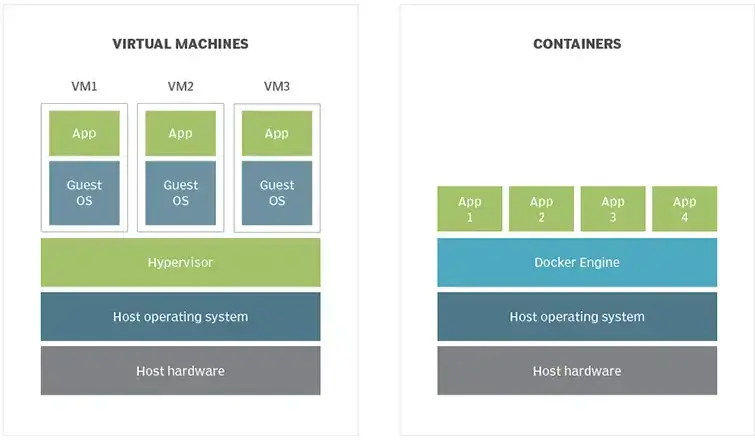
\includegraphics[width=0.85\textwidth]{imagenes/cap3/maquina-virtual-vs-contenedor.png}
    \caption{Comparación entre la arquitectura de una máquina virtual y la de un contenedor. Fuente: \url{https://electronicaonline.net/software-y-apps/windows/maquina-virtual/}}
    \label{fig:vm_vs_container}
\end{figure}

Desde el punto de vista de la gestión, los contenedores ofrecen despliegues más rápidos (menos de un segundo frente a decenas de segundos en VMs) y una mayor flexibilidad en la asignación de recursos. Sin embargo, la migración en vivo está más desarrollada en VMs, mientras que en contenedores se encuentra en una etapa menos madura. Asimismo, el desarrollo de software se ve favorecido en los contenedores gracias a la construcción más rápida de imágenes, menor tamaño de almacenamiento y capacidades integradas de control de versiones \cite{sharma2016containers}.

\begin{table}[ht]
    \centering
    \begin{tabular}{p{4cm} p{4cm} p{4cm}}
        \toprule
        \textbf{Característica}         & \textbf{Máquinas virtuales} & \textbf{Contenedores}        \\
        \midrule
        Aislamiento                     & Completo                    & Parcial (kernel compartido)  \\
        Consumo de recursos             & Alto                        & Bajo                         \\
        Tiempo de arranque              & Largo                       & Corto                        \\
        Portabilidad                    & Alta                        & Muy alta                     \\
        Acceso a hardware especializado & Limitado                    & Directo con soporte adecuado \\
        Mantenimiento y despliegue      & Complejo                    & Simple                       \\
        Rendimiento en CPU              & Casi nativo                 & Casi nativo                  \\
        Rendimiento en memoria          & Degradación $\sim$10\%      & Mejor que VMs                \\
        Rendimiento en E/S de disco     & Hasta 80\% peor             & Cercano a nativo             \\
        \bottomrule
    \end{tabular}
    \caption{Comparativa entre máquinas virtuales y contenedores en entornos HPC, incluyendo resultados de Sharma et al. (2016)~\cite{sharma2016containers}.}
    \label{tab:vm_vs_container}
\end{table}

En entornos HPC, la contenerización se ha consolidado como la opción preferida para aplicaciones que requieren eficiencia, portabilidad y reproducibilidad.

\subsection{Ecosistema de contenedores en HPC}\label{subsec:ecosistema_contenedores}

El ecosistema de contenedores en \acs{HPC} ha experimentado una evolución acelerada en los últimos años, motivado por la necesidad de incrementar la portabilidad, reproducibilidad y facilidad de despliegue de aplicaciones científicas y de ingeniería. Han surgido múltiples tecnologías y frameworks que ofrecen soluciones adaptadas, en mayor o menor medida, a los entornos HPC. Cada uno presenta ventajas, limitaciones y un grado diferente de adopción dentro de la comunidad científica.

\subsubsection{Docker}

Docker es la plataforma de contenedores más extendida a nivel global, reconocida por su capacidad para empaquetar aplicaciones junto con todas sus dependencias en imágenes portables, ejecutables en diferentes sistemas operativos y arquitecturas. Esta característica ha sido clave para su éxito, ya que permite reproducir entornos de software de manera consistente y simplifica considerablemente el despliegue y la gestión de aplicaciones.

Entre sus principales ventajas se encuentra la virtualización ligera a nivel de sistema operativo, que permite ejecutar contenedores de forma rápida y eficiente, sin la sobrecarga que implican las máquinas virtuales tradicionales. Esto conlleva un menor consumo de recursos y un arranque mucho más rápido, al compartir el kernel y las bibliotecas del host. Además, Docker facilita la portabilidad extrema, permitiendo mover aplicaciones entre distintos sistemas Linux sin inconsistencias, y asegura aislamiento y seguridad, evitando que contenedores independientes interfieran entre sí y eliminando residuos tras su eliminación.

Docker también contribuye a la reducción de costos y tiempos de despliegue, al eliminar configuraciones complejas y ofrecer entornos listos para ejecutar en cuestión de segundos. Su naturaleza de código abierto y gratuita elimina la necesidad de licencias comerciales, y su compatibilidad con arquitecturas de microservicios y herramientas de orquestación, como Kubernetes, simplifica la escalabilidad y la gestión de aplicaciones distribuidas \cite{Bhatia2017THERT}.

A pesar de estas ventajas, su uso en entornos HPC presenta ciertas limitaciones. La necesidad de permisos de root para ejecutar contenedores y las estrictas políticas de seguridad en clústeres multiusuario restringen su adopción, motivando el uso de alternativas como Podman o Singularity en contextos de computación de alto rendimiento.

\subsubsection{Podman}

Podman se presenta como una alternativa a Docker, compatible con la mayoría de sus comandos y formatos de imagen, pero con una diferencia fundamental: no requiere privilegios de root para la ejecución de contenedores. Esta característica lo hace especialmente adecuado para entornos HPC multiusuario, donde las políticas de seguridad son estrictas.

Entre sus ventajas, destaca el modo rootless, que permite ejecutar y construir contenedores sin privilegios administrativos, aislando el entorno del usuario y reduciendo los riesgos de escalada de privilegios. Podman también soporta múltiples runtimes, como \texttt{runc} y \texttt{crun}, y es compatible con el estándar OCI, lo que facilita la creación y utilización de imágenes en distintos entornos.

Otra característica importante es su modelo fork-exec sin daemon, que prescinde de un demonio central. Esto simplifica la auditoría y el control de recursos, alineándose con la filosofía de HPC. Además, en pruebas con aplicaciones reales y benchmarks estándar de CPU y memoria, Podman muestra un overhead muy bajo, comparable al de Singularity y Shifter \cite{gantikow2020rootless, stephey2022scaling}, lo que garantiza un rendimiento cercano al de ejecuciones \textit{bare-metal}, es decir, directamente sobre el hardware sin capas de virtualización adicionales.

Podman permite agrupar contenedores mediante Pods, compartiendo namespaces y facilitando la ejecución de aplicaciones complejas en paralelo. También optimiza el uso de recursos a gran escala, ya que el modo \textit{exec} para MPI minimiza el overhead de arranque y mejora el rendimiento en aplicaciones intensivas en metadatos. Asimismo, integra soporte para GPU y redes HPC avanzadas mediante hooks OCI y wrappers, permitiendo configurar librerías, variables de entorno y acceso a interconexiones de alta velocidad, como Cray Slingshot u otras equivalentes.

Por último, Podman facilita la gestión de usuarios y almacenamiento, ofreciendo subuid/subgid persistentes y almacenamiento local en los nodos de login, lo que mejora los tiempos de construcción de imágenes y la productividad de los usuarios. En conjunto, estas características hacen de Podman una herramienta versátil y eficiente para entornos HPC modernos.

Gracias a estas capacidades, Podman se posiciona como una alternativa robusta y escalable para la contenerización en HPC. Su modo rootless, rendimiento competitivo y soporte para entornos distribuidos lo convierten en una opción cada vez más valorada en centros de supercomputación y laboratorios de investigación \cite{gantikow2020rootless, stephey2022scaling}.

\subsubsection{Comparativa y adopción en la comunidad científica}

En función de su adopción y casos de uso, destacan los siguientes puntos:

\subsubsection{Comparativa y adopción en la comunidad científica}

En la práctica, Docker y Podman se utilizan en contextos distintos dentro de la comunidad científica. Docker es ampliamente empleado en desarrollo y pruebas debido a su ecosistema maduro, la virtualización ligera, la portabilidad y la eficiencia en el uso de recursos \cite{Bhatia2017THERT}. Por su parte, Podman ha ganado popularidad en entornos HPC, gracias a su ejecución rootless, su rendimiento a escala comparable al de ejecuciones \textit{bare-metal} y su compatibilidad con \textit{runtimes} modernos \cite{gantikow2020rootless, stephey2022scaling}.

Esta diferenciación refleja cómo la comunidad científica selecciona la herramienta más adecuada según el tipo de carga de trabajo y las restricciones de seguridad de cada entorno.

\subsubsection{Retos principales en la contenerización en HPC}

La computación de alto rendimiento presenta desafíos específicos que afectan tanto a la eficiencia como a la adopción de tecnologías emergentes como la contenerización \cite{zhou2022containerisation}. Uno de los principales obstáculos es la compatibilidad de software y librerías. La coexistencia de distintas versiones de librerías, como \textit{glibc}, o diferencias en el ABI del kernel pueden generar fallos o comportamientos inesperados. Además, no todas las imágenes de Docker son directamente portables a otros motores de contenedores utilizados en HPC, debido a la falta de estandarización completa en los hooks de ejecución y en la gestión de privilegios.

La seguridad constituye otro reto importante. En entornos HPC, los contenedores comparten el mismo kernel, lo que hace que vulnerabilidades en uno de ellos puedan comprometer la estabilidad del sistema completo. Amenazas como la escalada de privilegios, ataques de denegación de servicio (DoS) o fugas de información son preocupantes. Aunque mecanismos como los \textit{cgroups} y los \textit{user namespaces} ayudan a mitigar estos riesgos, muchos centros de supercomputación optan por deshabilitarlos parcialmente, lo que limita la adopción de contenedores modernos.

Otro desafío es la posible degradación del rendimiento. La ejecución de aplicaciones dentro de contenedores puede afectar la eficiencia, especialmente cuando se utilizan librerías optimizadas para GPUs o interconexiones de alta velocidad, como InfiniBand. Asimismo, al incrementar el número de procesos MPI en un mismo nodo, los costes de comunicación interna aumentan, afectando tanto a operaciones punto a punto como colectivas.

Finalmente, los contenedores presentan limitaciones en la personalización del kernel. A diferencia de los entornos nativos, restringen la instalación de módulos de kernel para preservar el aislamiento, lo que impide realizar ajustes de bajo nivel que podrían mejorar el rendimiento en escenarios HPC. Aunque existen propuestas experimentales como \textit{Xcontainer}, estas todavía no están maduras para un uso generalizado.

\subsection{Limitaciones de la contenerización en macOS}

El uso de contenedores en macOS presenta desafíos específicos, especialmente en lo que respecta al acceso y aprovechamiento de la GPU. A diferencia de los entornos Linux, donde los contenedores pueden habilitar el acceso directo a dispositivos de hardware, en macOS existen restricciones derivadas de la arquitectura del sistema y de la infraestructura de virtualización utilizada por Docker. Estas limitaciones afectan de manera significativa a aplicaciones de HPC y de inteligencia artificial que requieren aceleración por GPU, dificultando su ejecución eficiente y restringiendo el rendimiento alcanzable en este sistema operativo.

Uno de los principales obstáculos es la ausencia de soporte para GPU passthrough. Docker en macOS no permite el acceso directo a la GPU del host, lo que impide que los contenedores aprovechen la aceleración por hardware y limita el rendimiento de aplicaciones que dependen de procesamiento gráfico intensivo o cómputo acelerado. Esta restricción está estrechamente vinculada a la dependencia de la infraestructura de virtualización de Apple, la cual no proporciona acceso nativo a la GPU, afectando negativamente tanto el rendimiento como la compatibilidad de aplicaciones científicas y de ingeniería.

Aunque existen alternativas como Vulkan o MoltenVK que permiten cierto grado de aceleración gráfica en contenedores sobre macOS, el rendimiento obtenido es notablemente inferior al que se logra en entornos Linux o Windows. Además, la configuración de estas tecnologías suele ser compleja y no garantiza compatibilidad total con todas las aplicaciones. En general, habilitar el acceso a la GPU en contenedores sobre macOS enfrenta desafíos técnicos importantes, derivados de la infraestructura de virtualización y de la falta de soporte oficial para GPU passthrough.

En conjunto, estos retos muestran que, si bien la contenerización aporta ventajas claras en términos de reproducibilidad, portabilidad y flexibilidad, su implementación en macOS requiere soluciones específicas para gestionar dependencias, garantizar la seguridad en entornos compartidos y mantener la eficiencia en hardware y comunicaciones paralelas. Muchas de estas cuestiones siguen siendo áreas activas de investigación dentro de la comunidad HPC.

\section{Portabilidad y reproducibilidad científica}\label{sec:portabilidad_reproducibilidad}

La portabilidad y la reproducibilidad son aspectos fundamentales en la computación científica moderna. La creciente heterogeneidad de plataformas, que abarca desde supercomputadores tradicionales hasta infraestructuras en la nube o clústeres híbridos CPU-GPU, dificulta que una aplicación pueda ejecutarse sin modificaciones en distintos entornos. Además, la reproducibilidad de resultados experimentales se ha convertido en un reto central, ya que incluso pequeñas diferencias en el entorno de ejecución pueden conducir a variaciones significativas en los resultados obtenidos.

En este contexto, la contenerización emerge como una solución tecnológica que no solo aporta ventajas en términos de gestión e infraestructura, sino que también permite garantizar que las aplicaciones sean fácilmente portables y que los experimentos científicos puedan reproducirse bajo condiciones controladas y consistentes.

\subsection{Cómo los contenedores facilitan la portabilidad de aplicaciones HPC}

En el contexto de \acs{HPC}, la portabilidad se refiere a la capacidad de ejecutar una misma aplicación en diferentes sistemas de cómputo sin necesidad de modificar su código fuente ni su configuración. Los contenedores facilitan esta portabilidad al encapsular la aplicación junto con todas sus dependencias, incluyendo bibliotecas, compiladores, intérpretes, librerías de comunicación como MPI y entornos de ejecución específicos. De esta manera, se reduce significativamente la fricción que surge cuando un código funciona en un sistema pero falla en otro.

Mediante la creación de una única imagen de contenedor, es posible desplegar la misma aplicación en múltiples entornos, siempre que exista soporte para la tecnología de contenedores utilizada. Esto asegura consistencia entre plataformas, ya que el mismo contenedor puede ejecutarse en distintos sistemas operativos y arquitecturas, minimizando incompatibilidades. Asimismo, disminuye el tiempo de despliegue, ya que los usuarios no necesitan adaptar ni recompilar el software para cada infraestructura, y facilita el acceso a entornos heterogéneos que combinan CPUs y GPUs, donde la gestión de drivers y librerías suele ser crítica. Otro beneficio es la compatibilidad con diversos entornos, desde clusters virtuales autoescalables en la nube hasta infraestructuras HPC tradicionales o equipos personales, garantizando un entorno reproducible y consistente \cite{Vaillancourt2020SelfScalingCA}.

Además, el uso de gestores de paquetes como Nix dentro de contenedores permite fijar versiones exactas de bibliotecas y dependencias, asegurando lo que se denomina \textit{pureza funcional}. Esto garantiza que cualquier ejecución posterior del contenedor produzca resultados idénticos, independientemente de la plataforma en la que se ejecute \cite{Vaillancourt2020SelfScalingCA}.

\subsection{Reproducibilidad de experimentos científicos usando contenedores}

La reproducibilidad científica implica que los resultados de un experimento puedan replicarse bajo las mismas condiciones. En computación científica, factores como la evolución de bibliotecas, diferencias entre compiladores o cambios en sistemas operativos suelen comprometer esta reproducibilidad, dificultando la verificación de resultados a lo largo del tiempo.

Los contenedores abordan estos problemas al encapsular no solo el código de la aplicación, sino también todo el contexto de ejecución. De este modo, se puede garantizar que los experimentos se ejecuten en entornos idénticos, independientemente de la infraestructura subyacente. Por ejemplo, mediante tecnologías como Nix dentro de Docker o Singularity, es posible fijar versiones exactas de paquetes y librerías, asegurando reproducibilidad incluso años después \cite{Vaillancourt2020SelfScalingCA}.

Otra ventaja es la transparencia: al compartir la imagen del contenedor junto con el código y los datos, otros investigadores pueden verificar que los resultados se obtuvieron en condiciones equivalentes. Esto facilita también la colaboración eficiente entre equipos distribuidos geográficamente, que pueden trabajar sobre un mismo entorno sin necesidad de configurar individualmente cada sistema.

Asimismo, los contenedores reducen la carga administrativa. El uso de plantillas de contenedores (\textit{Container Template Library - CTL}) permite a los investigadores adaptar construcciones de software a sus necesidades, manteniendo la consistencia y la reproducibilidad sin depender de la intervención de administradores de sistemas \cite{Vaillancourt2020SelfScalingCA}. Además, la metodología de contenerización ofrece escalabilidad y flexibilidad, permitiendo ejecutar los mismos experimentos desde computadoras personales hasta clusters HPC o nubes públicas, garantizando que los resultados sigan siendo reproducibles en cualquier infraestructura \cite{Vaillancourt2020SelfScalingCA}.

En conjunto, los contenedores, especialmente cuando se integran con gestores de paquetes como Nix y tecnologías HPC como Singularity, proporcionan un marco sólido para asegurar la reproducibilidad de resultados científicos y habilitar la computación científica en entornos diversos de manera eficiente y segura.